\documentclass[aspectratio=169]{beamer}

\usepackage{amsmath}
\usepackage{amssymb}
\usepackage{amsthm}
\usepackage[english]{babel}
\usepackage{csquotes}
\usepackage{graphicx}
\usepackage{verbatim}
\usepackage{listings}
\usepackage{float}
\usepackage{dsfont}
\usepackage{xcolor}

\usetheme{Madrid}

\title{Geometric Numerical Integration}
\author{Will Woolfenden}
\date{May 17, 2024}

\begin{document}

\maketitle

\begin{frame}{Hamiltonian Mechanics}
	We describe a problem on positions $q_i$ and momenta $p_i$ with Hamilton's equations: \pause
	\begin{align*}
		&\dot{q} = \dfrac{\partial H}{\partial p}
		&
		\dot{p} = \dfrac{-\partial H}{\partial q}&.	
	\end{align*} \pause
	The Hamiltonian $H$ is an invariant of the system. \pause
	Defining $x = (q_1 \mathellipsis q_d, p_1 \mathellipsis p_d)^\top$ we can state the problem in its general form
	\begin{equation*}
		\dot{x} = J \nabla H(x)
	\end{equation*}
	where $J$ is the symplectic matrix.
\end{frame}

\begin{frame}{Symplecticity}
	A flow $\Phi$ is symplectic if it satisfies
	\begin{equation*}
		\Phi^\top J \Phi = J.
	\end{equation*}
	If a problem is Hamiltonian then its analytical flow map is symplectic.
\end{frame}

\begin{frame}{Symplectic Methods} \pause
	The Symplectic Euler method, with flow $\Phi_h$, is
	\begin{equation*}
		\begin{pmatrix}
			q_{n+1} \\
			p_{n+1} 
		\end{pmatrix} = \begin{pmatrix}
			q_{n} \\
			p_{n}
		\end{pmatrix} + h J \nabla H(q_{n}, p_{n+1}).
	\end{equation*} \pause
	The St\"ormer-Verlet method, with flow $\Phi_{h/2}^* \circ \Phi_{h/2}$, is
	\begin{align*}
		p_{n+\frac{1}{2}} &= p_n - \frac{h}{2}\nabla_q H \left( q_n, p_{n+\frac{1}{2}} \right) \\
		q_{n+1} &= q_n + \frac{h}{2}\left( \nabla_p H \left( q_n, p_{n+\frac{1}{2}} \right) + \nabla_p H \left(q_{n+1}, p_{n+\frac{1}{2}} \right) \right) \\
		p_{n+1} &= p_{n+\frac{1}{2}} - \frac{h}{2} \nabla_q H \left( q_{n+1}, p_{n+\frac{1}{2}} \right).
	\end{align*} \pause
	If the Hamiltonian $H$ is separable, then these methods are explicit.
\end{frame}

\begin{frame}{Examples}
	\begin{figure}
		\centering
		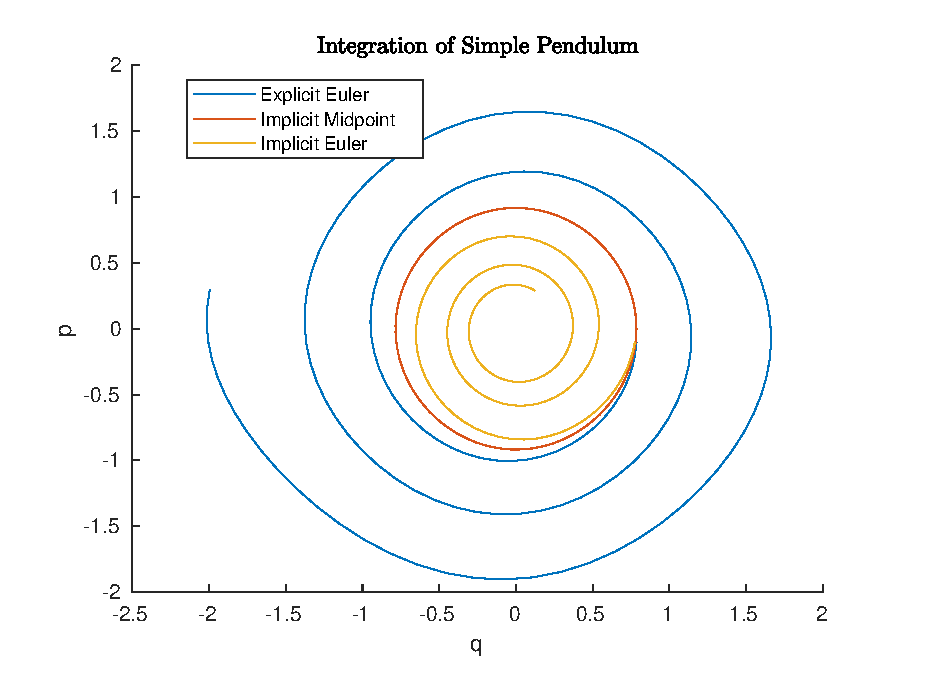
\includegraphics[height=0.7\textheight]{figures/pendulum.eps}
		\label{fig:pendulum}
	\end{figure}
\end{frame}

\begin{frame}{Examples}
	\begin{figure}
		\centering
		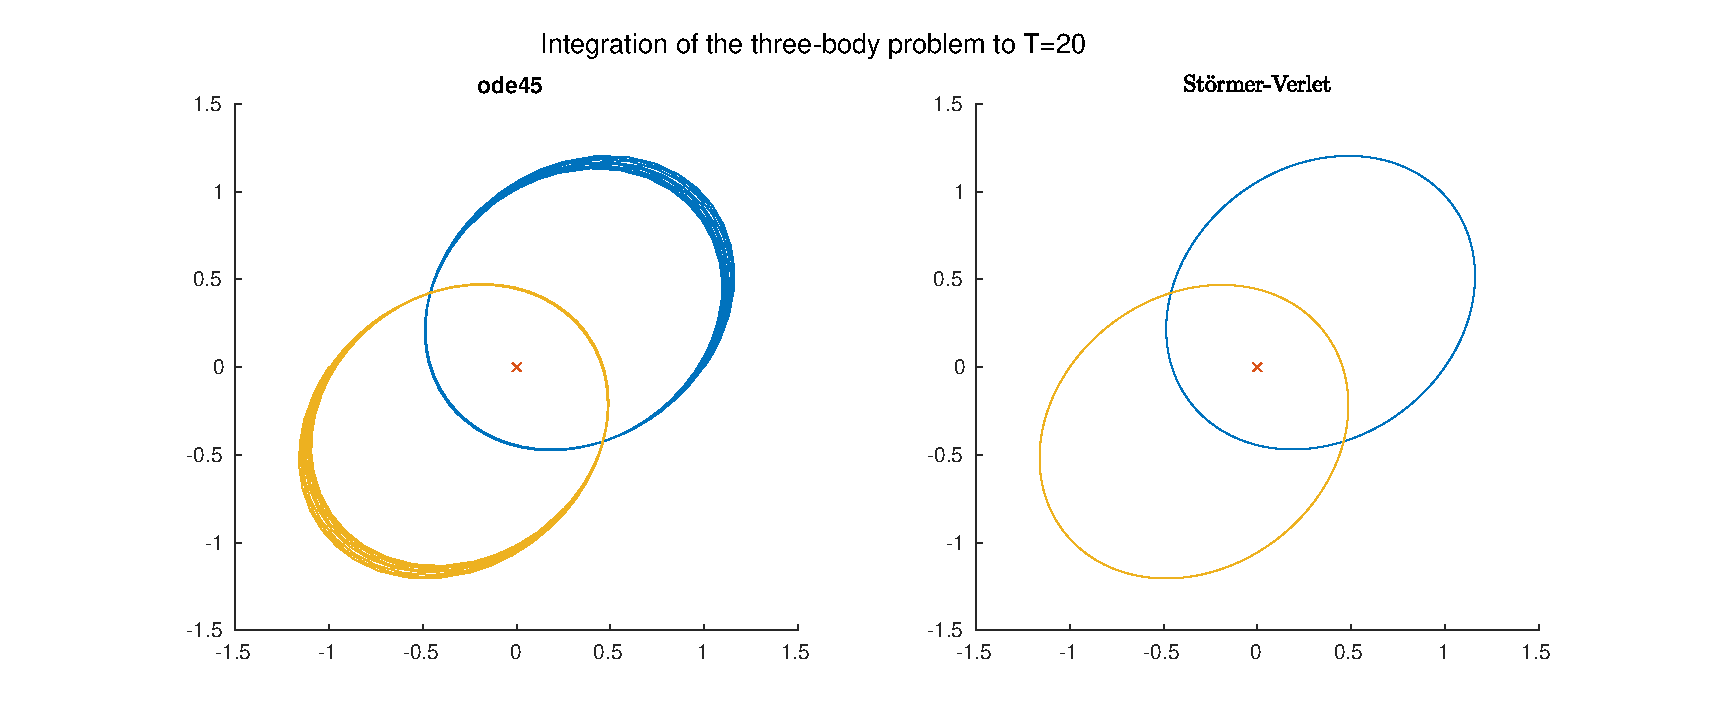
\includegraphics[width=\linewidth]{Matlab/threebodyorbit}
		\label{fig:threebody}
	\end{figure}
\end{frame}

\begin{frame}{Positivity Preservation}
	If a system is described using a graph-Laplacian matrix
	\begin{equation*}
		\dot{x} = A(t,x)x
	\end{equation*}
	then its solutions $x(t)$ preserve positivity. \\ \pause
	If a system is described using a constant matrix 
	\begin{equation*}
		\dot{x} = Bx
	\end{equation*}
	then it admits solutions $x(t) = \mathrm{e}^B x_0$. \\ \pause
	We can use this to produce a method
	\begin{equation*}
		x_{n+1} = \exp(h A(x_n)) x_n
	\end{equation*}
	which is first-order accurate and unconditionally positivity preserving.
\end{frame}

\begin{frame}{Positivity Preserving Integrators}
	Two second order methods of interest are \pause the strang splitting method
	\begin{equation*}
		\begin{aligned}
			x_{n+\frac{1}{2}} &= \exp \left[ \frac{h}{2} A(z_n) \right] x_n \\
			z_{n+1} &= \exp \left[ h A(x_{n+\frac{1}{2}}) \right] z_n \\
			x_{n+1} &= \exp \left[ \frac{h}{2} A(z_{n+1}) \right] x_{n+\frac{1}{2}}.
		\end{aligned}
		\label{eqn:secondorderstrangsplittingmethod}
	\end{equation*} \pause
	and the (midpoint) Magnus integrator
	\begin{equation*}
		x_{n+1} = \exp\left[h A \left( \exp\left[\frac{1}{2}h A(x_n)\right] x_n \right) \right] x_n.
		\label{eqn:secondordermagnus}
	\end{equation*}
	which are both positivity preserving.
\end{frame}

\begin{frame}{Approximating the Matrix Exponential}
	We may want to reduce the cost of computing the matrix exponential. \pause
	We focus on
	\begin{enumerate}
		\item<2-> series: $$\mathrm{e}^{hA} = \sum_{k=0}^{N} \frac{(hA)^k}{k!} + \mathcal{O}(h^{N+1})$$
		\item<3-> pad\'e: $$\mathrm{e}^{hA} = Q_{n,m}^{-1} P_{n,m} + \mathcal{O}(h^{n+m+1}).$$
	\end{enumerate}\pause[4]
	These approximations may need to be adjusted so they preserve positivity.
\end{frame}

\begin{frame}{Examples}
	\begin{figure}
		\centering
		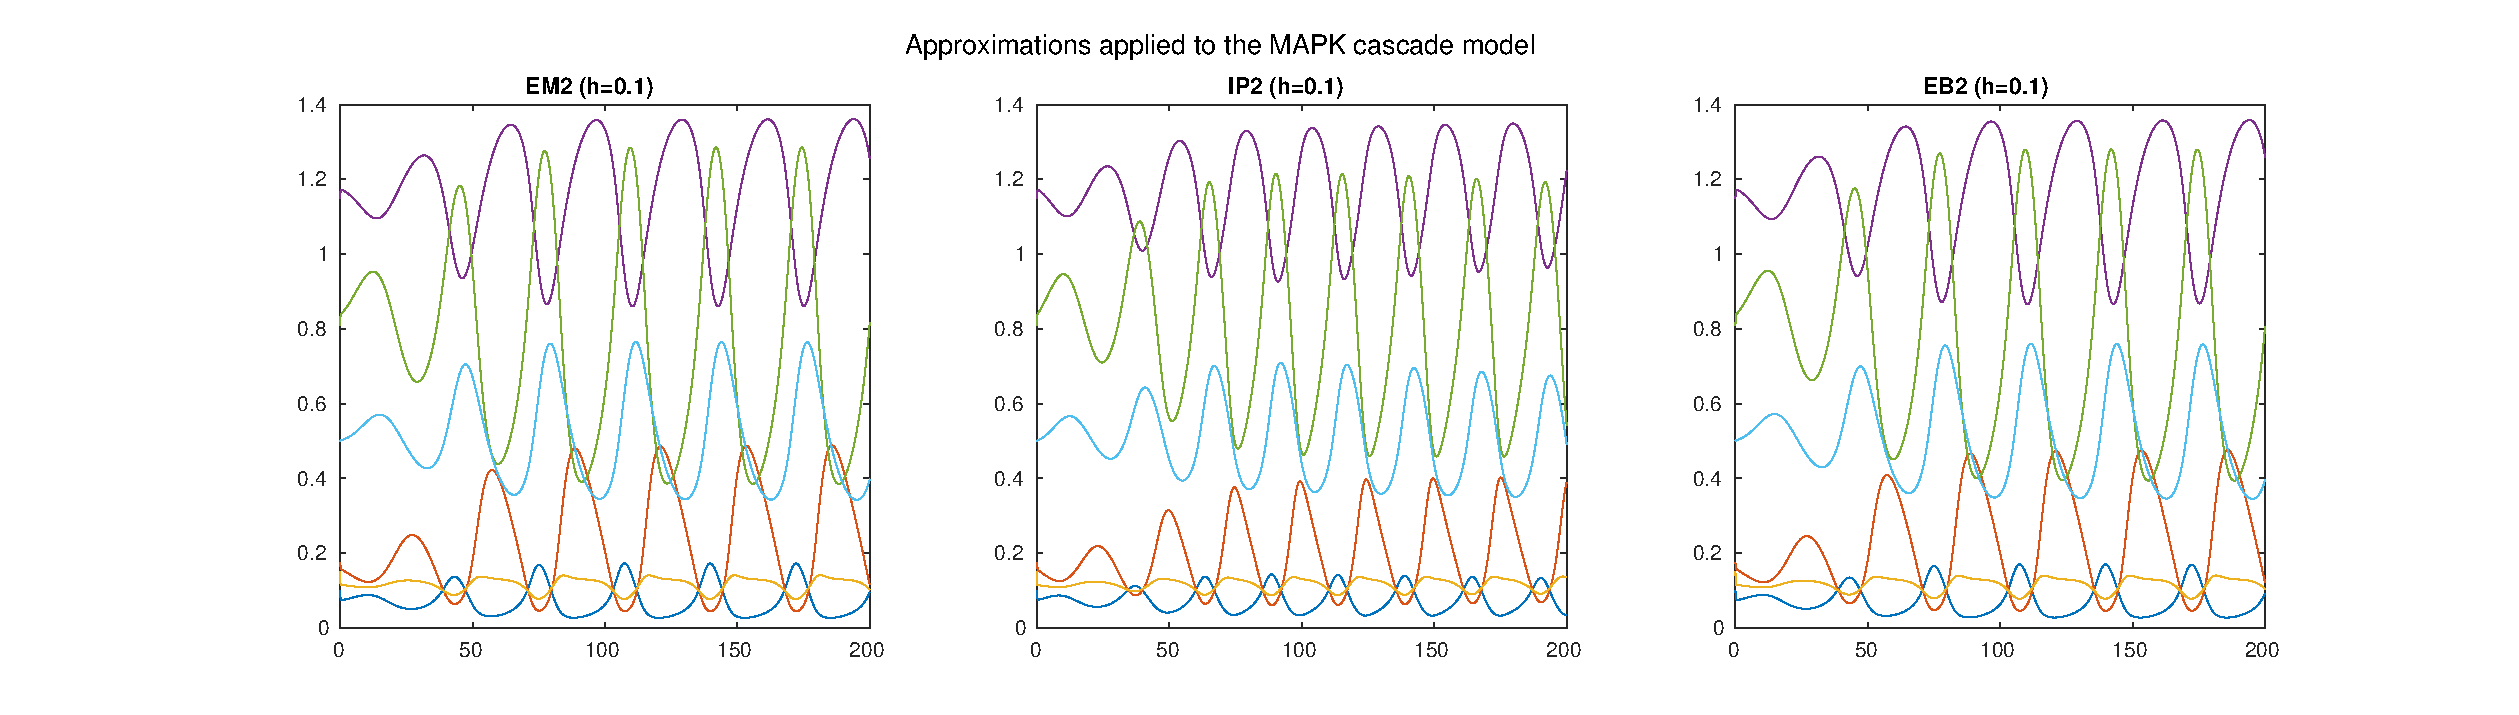
\includegraphics[width=\linewidth]{Matlab/magnustriplemapk.eps}
		\label{fig:triplemagnus}
	\end{figure}
\end{frame}

\begin{frame}{Examples}
	\begin{figure}
		\centering
		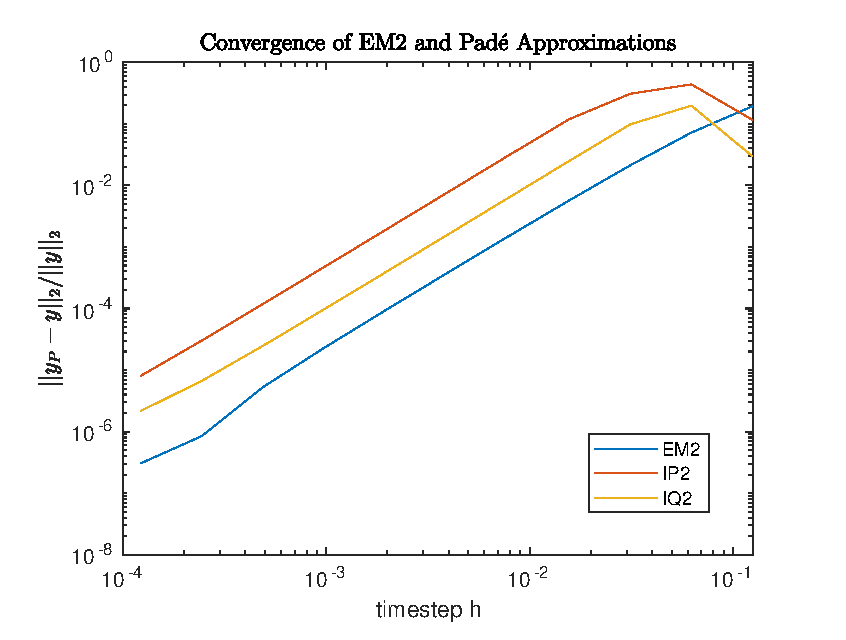
\includegraphics[width=0.5\linewidth]{Matlab/positivemapk2.eps}
		\label{fig:pademapkpos}
	\end{figure}
\end{frame}

\begin{frame}
	\centering
	Thank you for listening.
\end{frame}





\end{document}